\resizebox{\textwidth}{!}{%
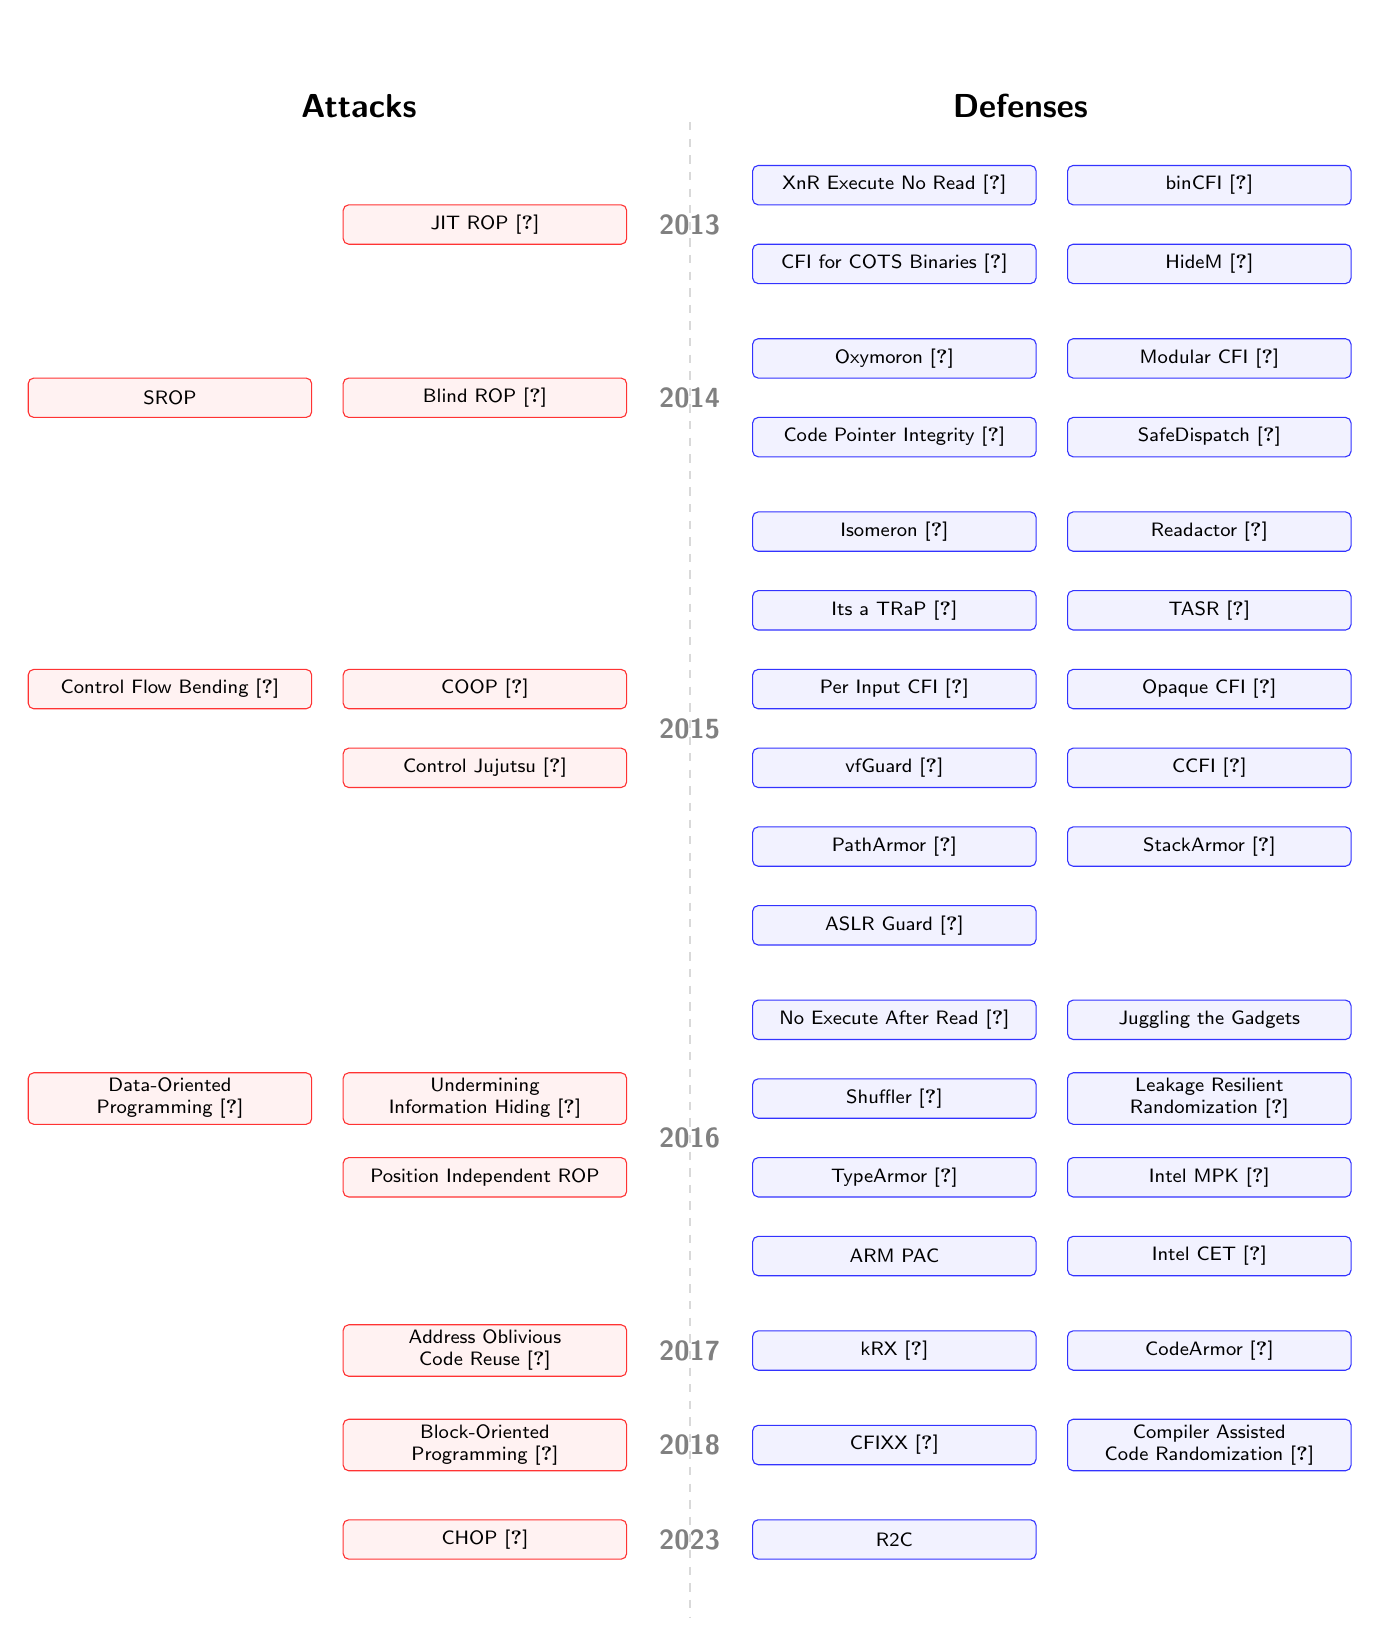
\begin{tikzpicture}[year node/.style={font=\bfseries\sffamily\color{gray}, align=center, inner sep=2pt},attack node/.style={draw=red!80, fill=red!5, rounded corners=2pt, font=\scriptsize\sffamily, align=center, minimum width=3.60cm, minimum height=0.5cm, inner sep=2pt, text width=3.40cm, execute at begin node=\setlength{\emergencystretch}{0pt}\tolerance 200\hyphenpenalty 10000\exhyphenpenalty 10000},defense node/.style={draw=blue!80, fill=blue!5, rounded corners=2pt, font=\scriptsize\sffamily, align=center, minimum width=3.60cm, minimum height=0.5cm, inner sep=2pt, text width=3.40cm, execute at begin node=\setlength{\emergencystretch}{0pt}\tolerance 200\hyphenpenalty 10000\exhyphenpenalty 10000},spine/.style={thick, gray!30, dashed}]%
\node[font=\large\bfseries\sffamily] at (-4.2,1.0) {Attacks};%
\node[font=\large\bfseries\sffamily] at (4.2,1.0) {Defenses};%
  % Year 2013%
\node[year node] at (0.0,-0.5) {2013};%
\node[attack node] at (-2.6,-0.5) {JIT ROP \allowbreak\cite{Snow2013}};%
\node[defense node] at (2.6,0.0) {XnR Execute No Read \allowbreak\cite{Backes2013}};%
\node[defense node] at (6.6,0.0) {binCFI \allowbreak\cite{zhang2013}};%
\node[defense node] at (2.6,-1.0) {CFI for COTS Binaries \allowbreak\cite{zhang2013}};%
\node[defense node] at (6.6,-1.0) {HideM \allowbreak\cite{Goktas2016b}};%
  % Year 2014%
\node[year node] at (0.0,-2.7) {2014};%
\node[attack node] at (-2.6,-2.7) {Blind ROP \allowbreak\cite{Bittau2014a}};%
\node[attack node] at (-6.6,-2.7) {SROP};%
\node[defense node] at (2.6,-2.2) {Oxymoron \allowbreak\cite{Backes2014f}};%
\node[defense node] at (6.6,-2.2) {Modular CFI \allowbreak\cite{niu2014a}};%
\node[defense node] at (2.6,-3.2) {Code Pointer Integrity \allowbreak\cite{Kuznetsov2014}};%
\node[defense node] at (6.6,-3.2) {SafeDispatch \allowbreak\cite{jang2014}};%
  % Year 2015%
\node[year node] at (0.0,-6.9) {2015};%
\node[attack node] at (-2.6,-6.4) {COOP \allowbreak\cite{Schuster2015a}};%
\node[attack node] at (-6.6,-6.4) {Control Flow Bending \allowbreak\cite{Carlini2015a}};%
\node[attack node] at (-2.6,-7.4) {Control Jujutsu \allowbreak\cite{Evans2015a}};%
\node[defense node] at (2.6,-4.4) {Isomeron \allowbreak\cite{Davi2015}};%
\node[defense node] at (6.6,-4.4) {Readactor \allowbreak\cite{Crane2015}};%
\node[defense node] at (2.6,-5.4) {Its a TRaP \allowbreak\cite{Crane2015b}};%
\node[defense node] at (6.6,-5.4) {TASR \allowbreak\cite{bigelow2015}};%
\node[defense node] at (2.6,-6.4) {Per Input CFI \allowbreak\cite{Niu2015}};%
\node[defense node] at (6.6,-6.4) {Opaque CFI \allowbreak\cite{Mohan2015}};%
\node[defense node] at (2.6,-7.4) {vfGuard \allowbreak\cite{Prakash2015}};%
\node[defense node] at (6.6,-7.4) {CCFI \allowbreak\cite{Mashtizadeh2015}};%
\node[defense node] at (2.6,-8.4) {PathArmor \allowbreak\cite{Goktas2016b}};%
\node[defense node] at (6.6,-8.4) {StackArmor \allowbreak\cite{Chen2015c}};%
\node[defense node] at (2.6,-9.4) {ASLR Guard \allowbreak\cite{Lu2015}};%
  % Year 2016%
\node[year node] at (0.0,-12.1) {2016};%
\node[attack node] at (-2.6,-11.6) {Undermining\\ Information Hiding \allowbreak\cite{Goktas2016}};%
\node[attack node] at (-6.6,-11.6) {Data{-}Oriented\\ Programming \allowbreak\cite{Hu2016}};%
\node[attack node] at (-2.6,-12.6) {Position Independent ROP};%
\node[defense node] at (2.6,-10.6) {No Execute After Read \allowbreak\cite{Werner2016}};%
\node[defense node] at (6.6,-10.6) {Juggling the Gadgets};%
\node[defense node] at (2.6,-11.6) {Shuffler \allowbreak\cite{WilliamsKing2016}};%
\node[defense node] at (6.6,-11.6) {Leakage Resilient\\ Randomization \allowbreak\cite{Braden2016}};%
\node[defense node] at (2.6,-12.6) {TypeArmor \allowbreak\cite{VanderVeen2015b}};%
\node[defense node] at (6.6,-12.6) {Intel MPK \allowbreak\cite{Wahbe1993}};%
\node[defense node] at (2.6,-13.6) {ARM PAC};%
\node[defense node] at (6.6,-13.6) {Intel CET \allowbreak\cite{IntelCET}};%
  % Year 2017%
\node[year node] at (0.0,-14.8) {2017};%
\node[attack node] at (-2.6,-14.8) {Address Oblivious\\ Code Reuse \allowbreak\cite{Rudd2017}};%
\node[defense node] at (2.6,-14.8) {kRX \allowbreak\cite{Pomonis2019}};%
\node[defense node] at (6.6,-14.8) {CodeArmor \allowbreak\cite{Chen2017a}};%
  % Year 2018%
\node[year node] at (0.0,-16.0) {2018};%
\node[attack node] at (-2.6,-16.0) {Block{-}Oriented\\ Programming \allowbreak\cite{Ispoglou2018}};%
\node[defense node] at (2.6,-16.0) {CFIXX \allowbreak\cite{Burow2018CFIXX}};%
\node[defense node] at (6.6,-16.0) {Compiler Assisted\\ Code Randomization \allowbreak\cite{Koo2018}};%
  % Year 2023%
\node[year node] at (0.0,-17.2) {2023};%
\node[attack node] at (-2.6,-17.2) {CHOP \allowbreak\cite{duta2023}};%
\node[defense node] at (2.6,-17.2) {R2C};%
\path[spine,draw] (0.0,0.8) -- (0.0,-18.2);%
\path[use as bounding box] (-8.40,-18.20) rectangle (8.40,2.00);%
\end{tikzpicture}
}